\chapter{Planning final}
\label{ch:final}

Étant donné le changement de direction opéré, il a fallu corriger le planning.
La version présentée au préalable est valable en termes de délais mais des étapes ont changé.
Aussi, jusqu'en date du 19 juin, le planning reste valable.
Pour la suite du projet, en date du 19 juin 2020, un planning journalier sur deux semaines a été établi.
Il sera mis à jour et commenté de manière quotidienne afin de pouvoir affiner au maximum les différentes étapes journalière.
Aussi, une mise à jour hebdomadaire sera faite afin de garder deux semaines de planning effectif.
\newline

\begin{figure}[H]
	\centering
	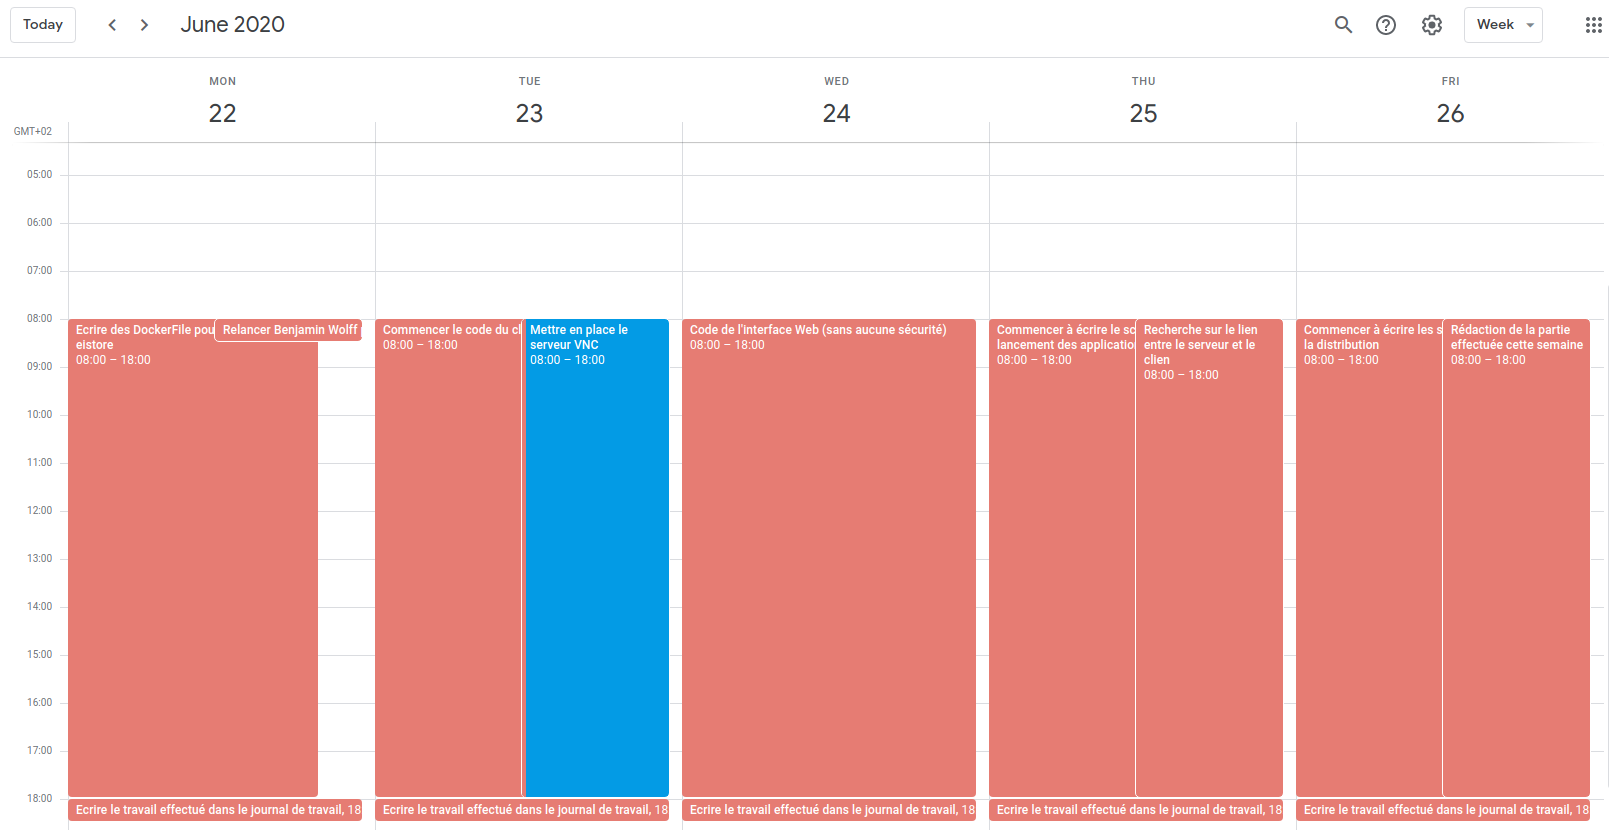
\includegraphics[scale=0.25]{images/planning/week1.png}
	\caption{Semaine 1 du travail à plein temps}
	\label{fig:week1}
\end{figure}


\begin{figure}[H]
	\centering
	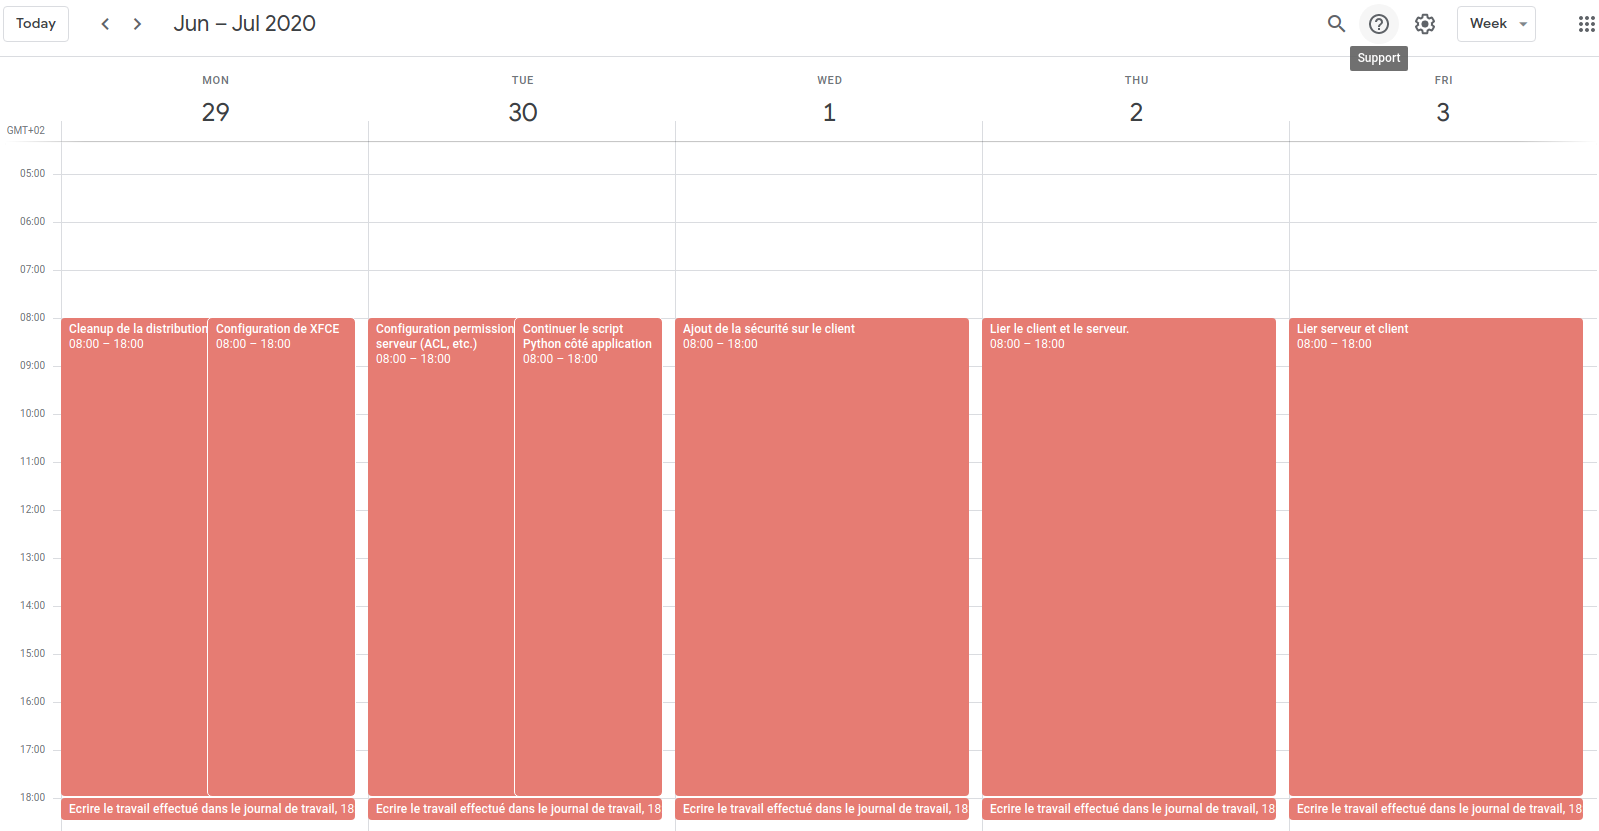
\includegraphics[scale=0.25]{images/planning/week2.png}
	\caption{Semaine 2 du travail à plein temps}
	\label{fig:week2}
\end{figure}


\begin{figure}[H]
	\centering
	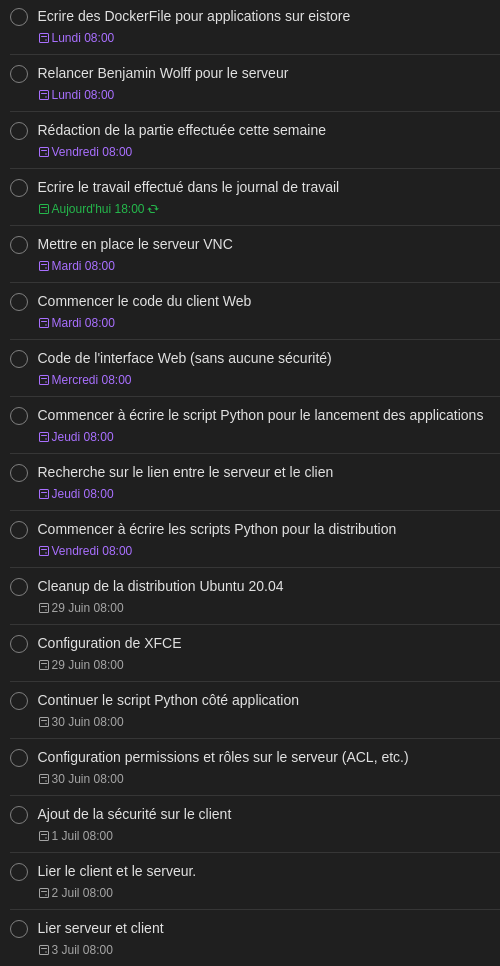
\includegraphics[scale=0.25]{images/planning/overview6Jul.png}
	\caption{Vue d'ensemble jusqu'au 6 juillet}
	\label{fig:ov6jul}
\end{figure}

